% Chapter Template

\chapter{Likelihood Model} % Main chapter title

\label{Likelihood Model} % Change X to a consecutive number; for referencing this chapter elsewhere, use \ref{ChapterX}

\lhead{Chapter 6. \emph{Likelihood Model}} % Change X to a consecutive number; this is for the header on each page - perhaps a shortened title

The likelihood model used for the results in \ref{results} (neglecting systematics) is given by   

\begin{equation}
  L_{hadronic} = \Pi Pois(n^i|b^i+s^i)
  \label{eq:likelihoodModel}
\end{equation}

where $n^i$ are the data, $b^i$ are the background predictions and $s^i$ are the signal predictions. The $b^i$ are predicted using electroweak control samples. Each prediction for a background source leads to a nuisance correlated in the NV dimension. These are modelled following a log normal distribution of mean 1 and width given by the systematic found through closure tests. Finally a log uniform systematic is assigned to account for the statistics in the control region.

All significances and limits are calculated using the asymptotic formulae described in \cite. A study was carried out into the reliability of this estimation and the results shown in \ref{asympToys}. As seen the differences between CLs toy and the asymptotic formulae are below 10\%.

\begin{figure}
  \centering
  %  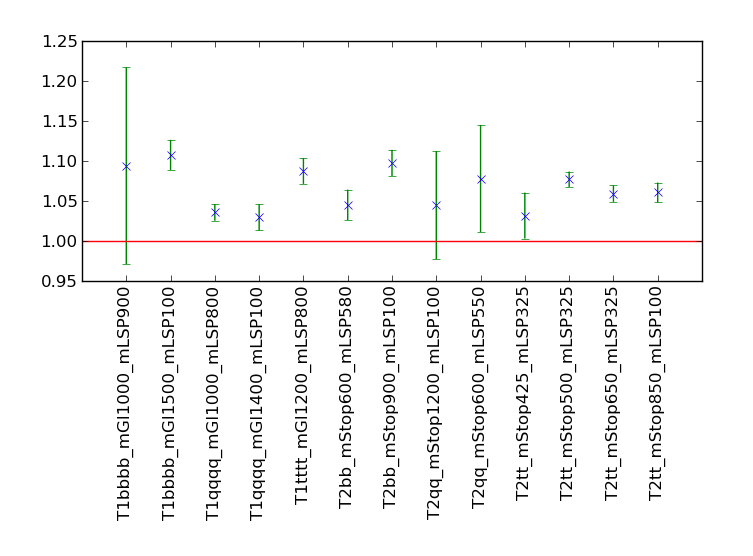
\includegraphics{Figures/asympToys.png}
     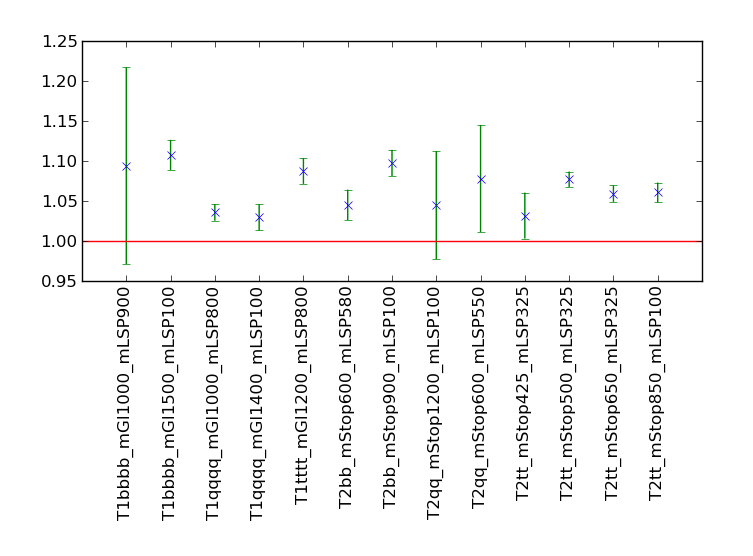
\includegraphics[width=0.7\textwidth]{Figures/asympToys.png}
  \caption{asympToys}
  \label{fig:asympToys}
\end{figure}
